\documentclass{bmvc2k}

%% Enter your paper number here for the review copy
% \bmvcreviewcopy{??}

% \usepackage[brazilian]{babel}
\usepackage[utf8]{inputenc}
\usepackage{listings}
\usepackage{amsmath}

\title{Mapa de profundidade\\ com câmeras estéreo}

% Enter the paper's authors in order
% \addauthor{Name}{email/homepage}{INSTITUTION_CODE}
\addauthor{Mateus Berardo de Souza Terra\\17/0018806}{mateus.b.s.terra@gmail.com}{1}
\addauthor{Víctor Rodrigues Pacheco\\17/0063879}{victorrpacheco98@gmail.com}{1}

% Enter the institutions
% \addinstitution{Name\\Address}
\addinstitution{
  Departamento de Ci\^encia da Comptuta\c{c}\~ao\\
  Universidade de Bras\'{\i}lia\\
  Campus Darcy Ribeiro, Asa Norte\\
  Bras\'{\i}lia-DF, CEP 70910-900, Brazil,  
}

\runninghead{Calibração de cameras}{Princípios da visão computacional 04/2019}

% Any macro definitions you would like to include
% These are not defined in the style file, because they don't begin
% with \bmva, so they might conflict with the user's own macros.
% The \bmvaOneDot macro adds a full stop unless there is one in the
% text already.
\def\eg{\emph{e.g}\bmvaOneDot}
\def\Eg{\emph{E.g}\bmvaOneDot}
\def\etal{\emph{et al}\bmvaOneDot}

%-------------------------------------------------------------------------
% Document starts here
\usepackage{amsmath}
\begin{document}

\maketitle

\begin{abstract}
Mostrou-se o procedimento de criação de mapas de profundidade com base em imagens obtidas a partir de câmeras estéreo disponíveis em\\ \url{http://vision.middlebury.edu/stereo/data/scenes2014/}.\\
A criação do algoritimo fez uso da biblioteca multiplataforma OpenCV \cite{openCV}. Considerando que as imagens fornecidas foram tiradas com câmeras previamente calibradas e que as imagens foram retificadas o primeiro passo foi a aplicado a técnica SumAll \cite{SumOfAbsDif} para gerar o mapa de disparidade e logo em seguida permitir a síntese do mapa de profundidade.
\end{abstract}

%-------------------------------------------------------------------------
\section{Introdução}
\label{sec:intro}
 A soma das distâncias absolutas, também conhecida como L1\_norm, é um algoritmo que compara duas imagens, ou procura uma certa imagem em outra. Para o cálculo, é utilizada uma imagem de referência de tamanho w que é comparada pixel a pixel com uma janela de mesmo tamanho na segunda imagem. A distância absoluta é calculada por meio da diferença entre os valores de cores.
 
 Esse algoritmo pode ser utilizado para indicar a disparidade, demonstrada na figura \ref{fig:Disparidade}, de imagens estéreo, realizadas por duas câmeras(a), embora não seja o melhor algoritmo, uma vez que não lida bem com oclusões ou mesmo deslocamentos.
 
 \begin{figure}[!h]
    \centering
    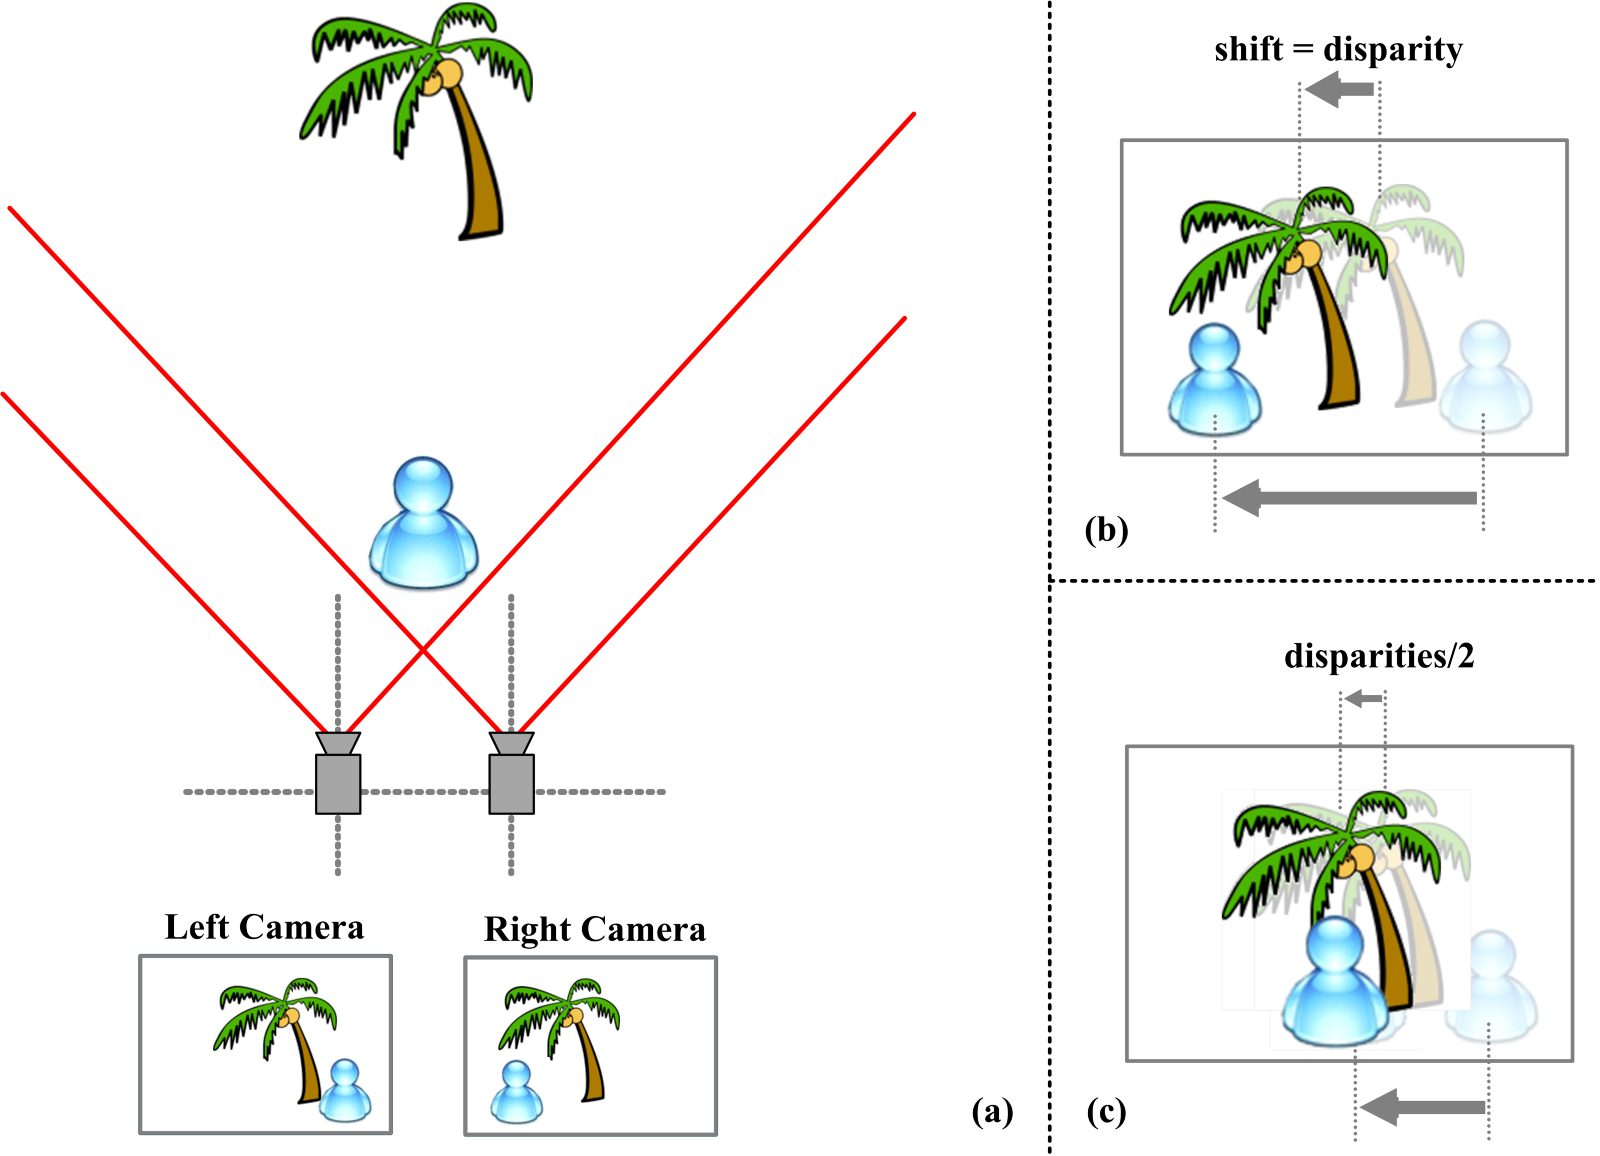
\includegraphics[width = 8cm]{Figs/StereoPicture.png}
    \caption{Disparidade.} 
    \label{fig:Disparidade}
   
    \url{https://cdn-images-1.medium.com/max/1600/1*wSyFon7Qm_DV165CZYMe8w.png}
\end{figure}


\subsection{Repositório}
O código desenvolvido nesse projeto estão, assim como o histórico de desenvolvimento, disponíveis na platafora GitHub em:


\url{https://github.com/MatTerra/StereoVision}.

\section{Desenvolvimento}
\label{sec:Desenvolvimento}
\subsection{Sistema}
Todos os códigos foram desenvolvidos e testados em uma máquina virtual Oracle VirtualBox \cite{VM} com as seguintes características e em um computador com as configurações descritas em seguida:
\begin{itemize}
    \item Versão VM 6.0.4
    \item Versão OS: Ubuntu 16.04 LTS 64-bits
    \item Versão Python: 3.5
    \item Versão OpenCV: 3.2.0
\end{itemize}

Segunda máquina:
\begin{itemize}
    \item Versão OS: Manjaro 18.04
    \item Versão Python: 3.5.6
    \item Versão OpenCV: 3.2.0
\end{itemize}

\section{Metodologia}
\label{sec:Metodologia}
\subsection{Requisito 1}
A execução deste requisito inicia pela implementação do algoritmo SAD. A implementação foi inicialmente testada na imagem Jade Plant, disponível em \cite{JadePlant}. 

Além da localização, utilizamos a biblioteca OpenCV para montar um mapa de disparidade das imagens. Testamos esse algoritmo nas duas imagens, obtendo melhores resultados na Motocicleta, disponível em\cite{Motorcycle}
 


\section{Resultados}
\subsection{SAD}
Com o SAD, processamos a imagem Jade Plant. Nela, o casamento de pontos não obteve resultados satisfatórios utilizando o SAD, embora a introdução de um offset na busca para restringir a busca a uma certa janela específica na imagem destino tenha melhorado os resultados.\\
Este offset foi baseado na distância média obtida manualmente entre pontos da imagem. Podemos ver um caso em que a busca é bem sucedida na figura \ref{fig:Resultado1OK} e outro caso em que a busca não retornou a posição correta na figura \ref{fig:Resultado1NOK}.

\subsection{Disparidade}
A escolha do número de disparidades e o mínimo valor que ela pode assumir criam um offset na imagem, ocasionando um bloco não processado. Na figura \ref{fig:disp}, podemos ver o mapa obtido para a cena da motocicleta \cite{Motorcycle}. É evidente que uma parte considerável da imagem não foi corretamente processada, sendo apenas ignorada. No mapa, pixels mais claros indicam maior disparidade.

\begin{figure}[htp]
    \centering
    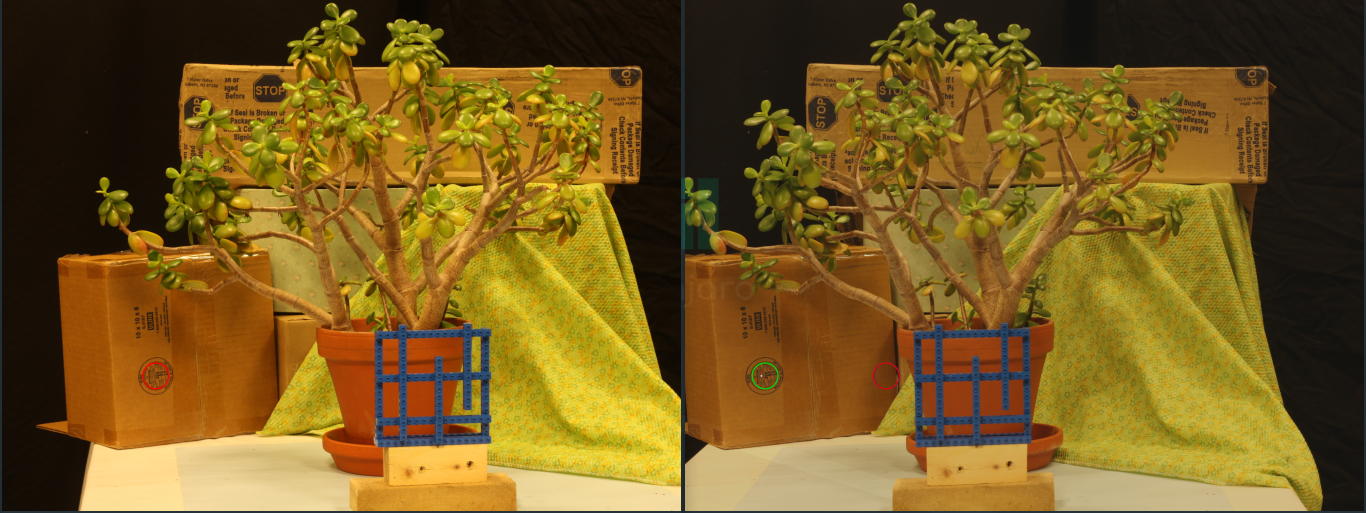
\includegraphics[width = 10cm]{Figs/Resultado1OK.png}
    \caption{Resultado 1 correto.}
    \label{fig:Resultado1OK}
\end{figure}

\begin{figure}[htp]
    \centering
    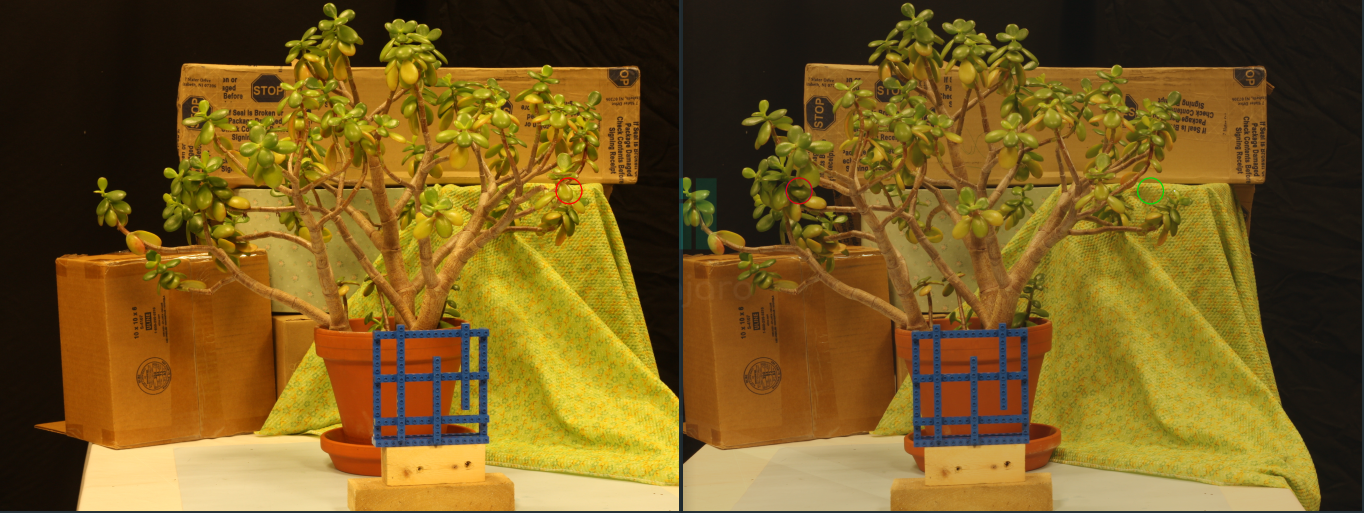
\includegraphics[width = 10cm]{Figs/Resultado1NOK.png}
    \caption{Resultado 1 não correto.}
    \label{fig:Resultado1NOK}
\end{figure}

\begin{figure}[htp]
    \centering
    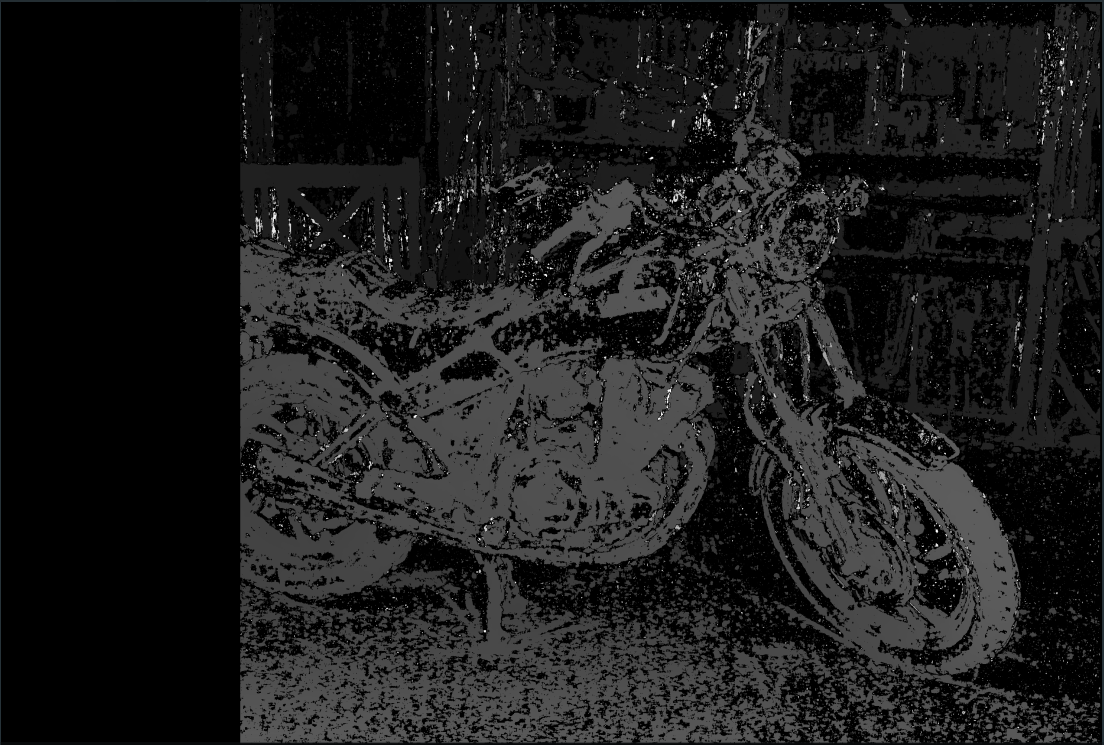
\includegraphics[width = 10cm]{Figs/DispMoto.png}
    \caption{Mapa de disparidade da motocicleta.}
    \label{fig:disp}
\end{figure}

\section{Conclusão}
Para a correta construção do mapa de profundidade são necessários 4 procedimentos:
\begin{itemize}
    \item Calibrar as câmeras;
    \item Retificar as imagens;
    \item Computar a Disparidade;
    \item Estimar a Profundidade.
\end{itemize}
Há dificuldade para a retificar as imagens e computar a disparidade principalmente por oscilações de brilho e pela presença de áreas de baixo contraste.\\
Foi notado também a impossibilidade de identificação da profundidade em áreas de oclusão (áreas capturadas apenas por uma câmera) pelo método adotado.


\bibliography{refs}
\end{document}
